\documentclass[a4paper,oneside,12pt]{report}
% Package yang diperlukan
\usepackage{graphicx}
\usepackage{geometry}
\usepackage{listings}
\usepackage{xcolor}
\usepackage{float}
\usepackage{hyperref}
\usepackage{natbib}
\usepackage{indentfirst}
\usepackage{url}
\usepackage{fancyhdr}
\usepackage{tocloft}
\usepackage{bookmark}

%======================================================================
% PENGATURAN GEOMETRI HALAMAN
%======================================================================
\geometry{left=3cm, right=2.5cm, top=2cm, bottom=2.5cm}
\sloppy

%======================================================================
% PENGATURAN WARNA UNTUK BLOK KODE
%======================================================================
\definecolor{codegreen}{rgb}{0,0.6,0}
\definecolor{codegray}{rgb}{0.5,0.5,0.5}
\definecolor{codepurple}{rgb}{0.58,0,0.82}
\definecolor{backcolour}{rgb}{0.95,0.95,0.92}
\definecolor{darkblue}{rgb}{0,0,0.6}

%======================================================================
% PENGATURAN BLOK KODE (LISTINGS)
%======================================================================
\lstdefinestyle{commonstyle}{
    backgroundcolor=\color{backcolour}, 
    breakatwhitespace=false, 
    breaklines=true, 
    captionpos=b, 
    keepspaces=true,
    numbers=left, 
    numbersep=5pt, 
    showspaces=false, 
    showstringspaces=false,
    showtabs=false, 
    tabsize=2, 
    frame=single,
    basicstyle=\ttfamily\footnotesize,
    numberstyle=\tiny\color{codegray},
    columns=flexible,
    postbreak=\mbox{\textcolor{red}{$\hookrightarrow$}\space},
    breakindent=0pt,
    breakautoindent=false
}

\lstdefinestyle{javastyle}{
    style=commonstyle,
    language=Java,
    commentstyle=\color{codegreen},
    keywordstyle=\color{darkblue}\bfseries,
    stringstyle=\color{codepurple},
    emph={@Test,@Mock,@InjectMocks,@ExtendWith,@BeforeEach,@AfterEach},
    emphstyle=\color{codepurple}
}

%======================================================================
% PENGATURAN LAIN-LAIN
%======================================================================
\renewcommand{\figurename}{Gambar}
\renewcommand{\thefigure}{\arabic{figure}}

\hypersetup{
    colorlinks=true, 
    linkcolor=black, 
    filecolor=black, 
    urlcolor=black,
    citecolor=blue,
    pdftitle={Laporan Praktikum}, 
    pdfpagemode=FullScreen, 
    breaklinks=true
}

\bibliographystyle{plain}

\pagestyle{fancy}
\fancyhf{}
\fancyfoot[C]{\thepage}
\renewcommand{\headrulewidth}{0pt}

\fancypagestyle{plain}{
    \fancyhf{}
    \fancyfoot[C]{\thepage}
    \renewcommand{\headrulewidth}{0pt}
}

%======================================================================
% PENGATURAN STRUKTUR BAB DAN DAFTAR ISI
%======================================================================
\renewcommand{\contentsname}{Daftar Isi}
\renewcommand{\bibname}{Daftar Pustaka}

\renewcommand{\thechapter}{}
\renewcommand{\chaptername}{}

\renewcommand{\thesection}{\arabic{chapter}.\arabic{section}}
\renewcommand{\thesubsection}{\thesection.\arabic{subsection}}

\setcounter{secnumdepth}{3}
\setcounter{tocdepth}{2}

\renewcommand{\cftchapdotsep}{\cftdotsep}
\renewcommand{\cftchapleader}{\cftdotfill{\cftchapdotsep}}
\setlength{\cftchapindent}{0em}
\setlength{\cftsecindent}{2em}
\setlength{\cftsubsecindent}{4em}
\setlength{\cftchapnumwidth}{0em}
\setlength{\cftsecnumwidth}{2.5em}
\setlength{\cftsubsecnumwidth}{3.2em}
\renewcommand{\cftchappresnum}{}
\renewcommand{\cftchapaftersnum}{}

\newcommand{\tocboldsection}[1]{%
  \protect\renewcommand{\protect\cftchapfont}{\protect\bfseries}%
  #1%
  \protect\renewcommand{\protect\cftchapfont}{}%
}

%======================================================================
% AWAL DOKUMEN
%======================================================================
\begin{document}

% Halaman Judul
\newgeometry{left=3cm, right=2.5cm, top=2.5cm, bottom=3cm}
\begin{titlepage}
\begin{center}
\vspace*{0.5cm}
{\large \textbf{\MakeUppercase{Laporan Praktikum}}} \\[0.4cm]
{\large \textbf{\MakeUppercase{PRAKTIKUM PENGUJIAN PERANGKAT LUNAK}}} \\[0.4cm]
{\large \textbf{\MakeUppercase{Pertemuan 10}}} \\[0.4cm]
{\large \textbf{\MakeUppercase{Page Object Model (POM)}}} \\[1.5cm]


\includegraphics[height=7cm]{lambang ugm.png} \\[1cm]

{\normalsize \textbf{Disusun oleh:}} \\[0.4cm]
\begin{tabular}{@{}l l @{}}
  \textbf{Nama}           & : Januarsyah Akbar \\
  \textbf{NIM}            & : 24/535846/SV/24314 \\
  \textbf{Kelas}          & : PL4B2 \\
  \textbf{Dosen Pengampu} & : Divi Galih Prasetyo Putri, S.Kom., M.Kom., Ph.D.
\end{tabular} \\[1.2cm]

{\normalsize \textbf{PROGRAM STUDI D-IV}} \\[0.2cm]
{\normalsize \textbf{TEKNOLOGI REKAYASA PERANGKAT LUNAK}} \\[0.2cm]
{\normalsize \textbf{DEPARTEMEN TEKNIK ELEKTRO DAN INFORMATIKA}} \\[0.2cm]
{\normalsize \textbf{SEKOLAH VOKASI}} \\[0.2cm]
{\normalsize \textbf{UNIVERSITAS GADJAH MADA}} \\[0.2cm]
{\normalsize \textbf{YOGYAKARTA}} \\[0.2cm]
{\normalsize \textbf{\today}} \\[1.2cm]
\end{center}
\end{titlepage}
\restoregeometry

\thispagestyle{empty}
\clearpage
\stepcounter{page}
\thispagestyle{empty}

% --- Daftar Isi ---
\addcontentsline{toc}{chapter}{Daftar Isi}
\tableofcontents
\clearpage

\pagenumbering{arabic}
\setcounter{page}{3}

%======================================================================
\chapter[Tujuan Praktikum]{Tujuan Praktikum}
%======================================================================
\begin{enumerate}
    \item Mahasiswa mampu memahami konsep \textit{Page Object Model} (POM).
    \item Mahasiswa mampu mengimplementasikan POM dalam skenario pengujian perangkat lunak di situs yang riil.
\end{enumerate}
\clearpage

%======================================================================
\chapter[\texorpdfstring{\tocboldsection{Hasil dan Pembahasan}}{Hasil dan Pembahasan}]{Hasil dan Pembahasan}
%======================================================================

%----------------------------------------------------------------------
\section{Latihan (POM pada Pencarian Bing)}
%----------------------------------------------------------------------

Pada bagian latihan ini, kita mengimplementasikan \textit{Page Object Model} (POM) untuk memisahkan logika skrip uji (\textit{test script}) dengan manajemen akses elemen web. Skenario yang digunakan adalah melakukan pencarian "janu ganteng" pada mesin pencari Bing, di mana strukturnya dibagi menjadi kelas \textit{Page} dan kelas Pengujian.

\subsection{Kelas \texttt{SearchPage}}
\begin{lstlisting}[style=javastyle, caption=Implementasi \texttt{SearchPage.java}]
package latihan;

import org.openqa.selenium.By;
import org.openqa.selenium.Keys;
import org.openqa.selenium.WebDriver;

public class SearchPage {
    private WebDriver driver;
    private By searchBox = By.name("q");

    public SearchPage(WebDriver driver) {
        this.driver = driver;
    }

    public void enterSearchQuery(String query) {
        driver.findElement(searchBox).sendKeys(query);
    }

    public void submitSearch() {
        driver.findElement(searchBox).sendKeys(Keys.ENTER);
    }
}
\end{lstlisting}
Kelas ini berisi inisialisasi \textit{locator} (seperti elemen kotak pencarian / \texttt{searchBox}) dan memberikan \textit{method} fungsionalitas bagi halaman utama (beranda pencarian) untuk menerima input dan menekan \textit{Enter}.

\subsection{Kelas \texttt{ResultPage}}
\begin{lstlisting}[style=javastyle, caption=Implementasi \texttt{ResultPage.java}]
package latihan;

import org.openqa.selenium.WebDriver;

public class ResultPage {
    private WebDriver driver;

    public ResultPage(WebDriver driver) {
        this.driver = driver;
    }

    public String getTitle() {
        return driver.getTitle();
    }
}
\end{lstlisting}
Kelas halaman kedua ini merepresentasikan rupa halaman interaksi ketika Bing telah menampilkan hasil. Skrip memusatkan pengaksesan elemen, yaitu pengambilan judul situs menggunakan metode \texttt{getTitle()}.

\subsection{Tahap Pengujian (\texttt{TestPage})}
\begin{lstlisting}[style=javastyle, caption=Implementasi \texttt{TestPage.java}]
package latihan;

import org.junit.jupiter.api.AfterEach;
import org.junit.jupiter.api.BeforeEach;
import org.junit.jupiter.api.Test;
import org.openqa.selenium.WebDriver;
import org.openqa.selenium.safari.SafariDriver;

import static org.junit.jupiter.api.Assertions.assertEquals;

public class TestPage {
    private WebDriver driver;
    private SearchPage searchPage;
    private ResultPage resultPage;

    @BeforeEach
    public void setUp() {
        driver = new SafariDriver();
        driver.manage().window().maximize();
        driver.get("https://www.bing.com/");
        
        searchPage = new SearchPage(driver);
        resultPage = new ResultPage(driver);
    }

    @Test
    public void testBingSearch() {
        String query = "janu ganteng";
        searchPage.enterSearchQuery(query);
        searchPage.submitSearch();

        try {
            Thread.sleep(2000);
        } catch (InterruptedException e) {
            e.printStackTrace();
        }

        assertEquals("janu ganteng - Search", resultPage.getTitle());
    }

    @AfterEach
    public void tearDown() {
        if (driver != null) {
            driver.quit();
        }
    }
}
\end{lstlisting}
Blok \texttt{TestPage} berlaku murni sebagai manajer jalannya pengujian. \texttt{WebDriver} dieksekusi di MacOS menggunakan \texttt{SafariDriver}. Seluruh kode \textit{boilerplate} terkait identifikasi \textit{tag} HTML tidak lagi berserakan berkat model POM, sehingga asersi akhir cukup memeriksa properti \textit{title} halaman.

\begin{figure}[H]
    \centering
    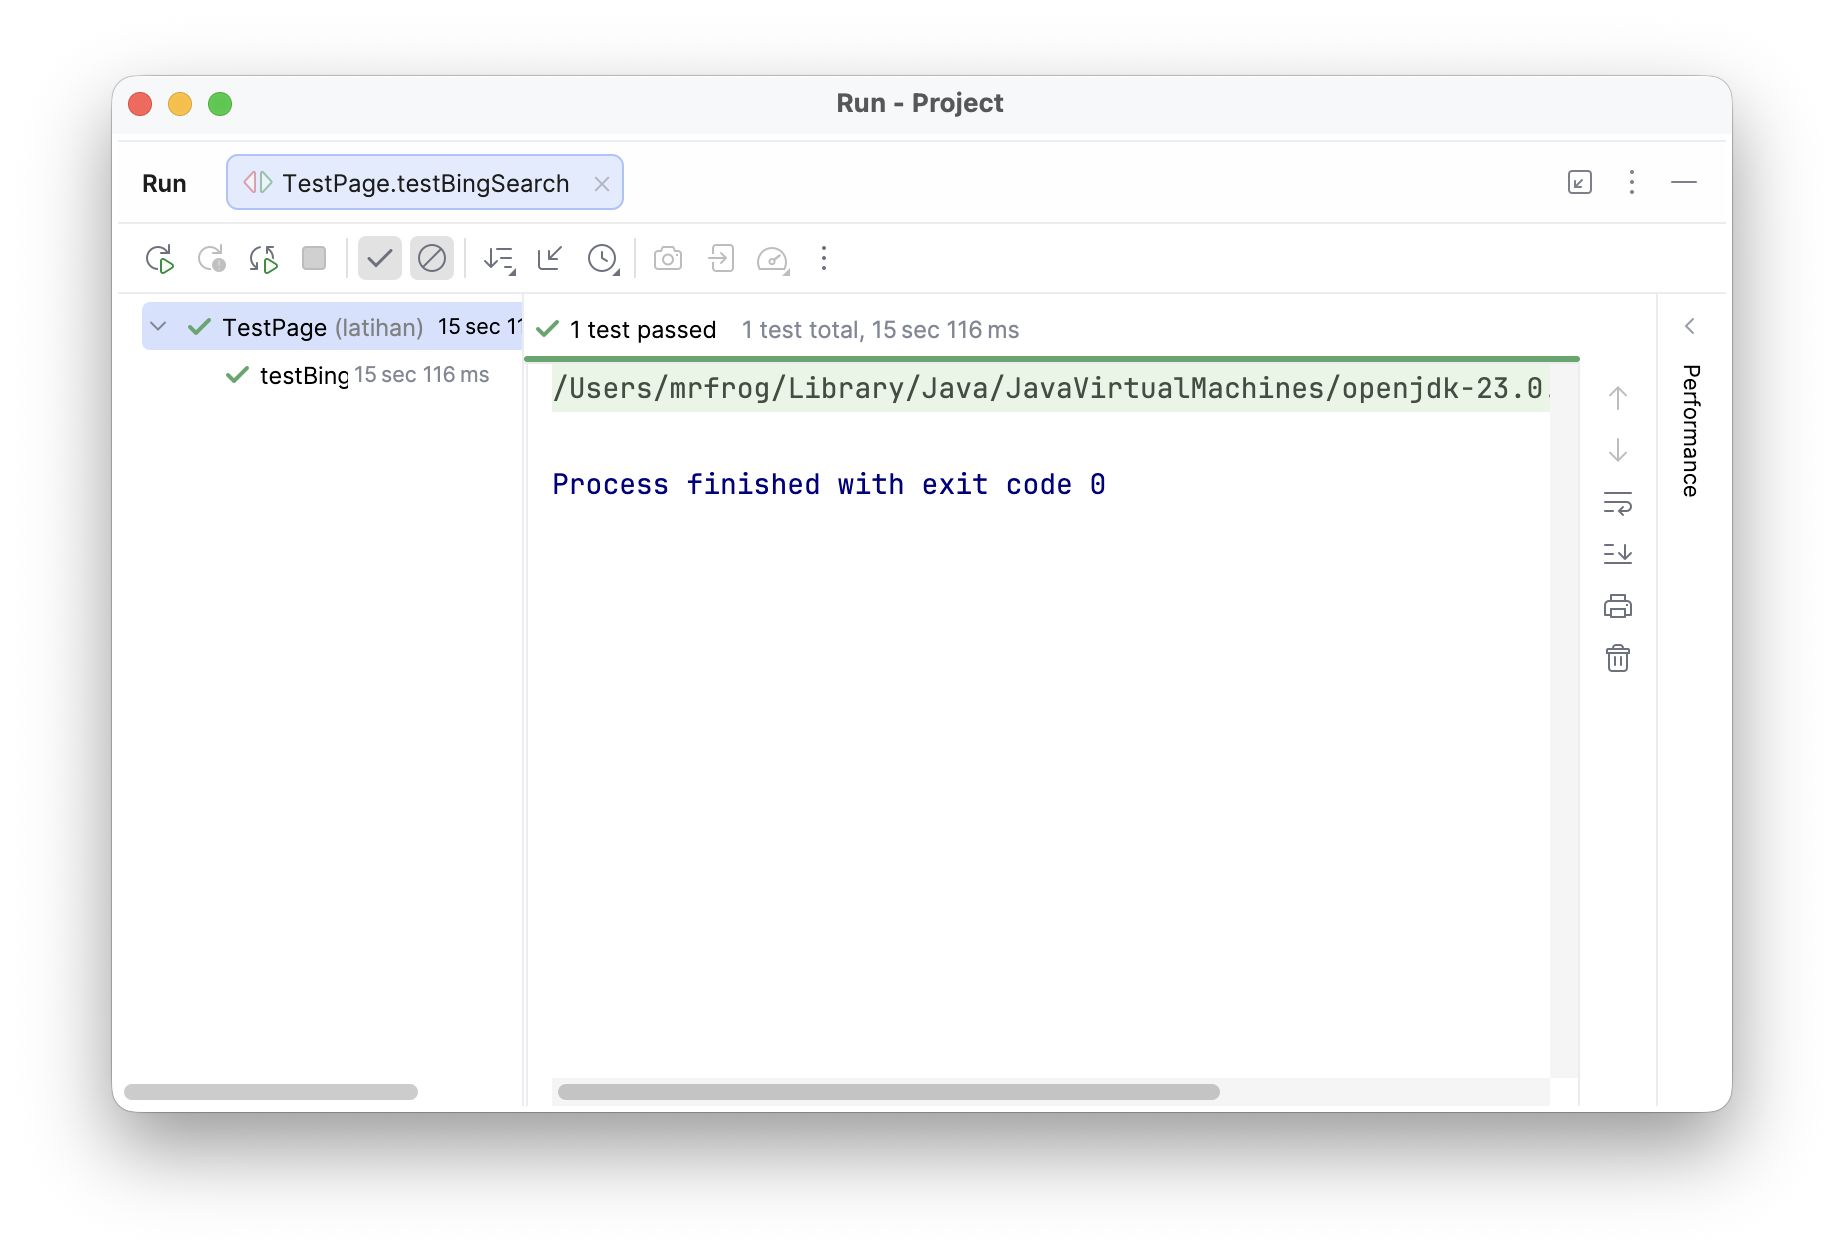
\includegraphics[width=0.9\textwidth]{screenshot step/Latihan_test_result.png}
    \caption{Bukti Hasil Eksekusi Selenium Latihan POM}
\end{figure}

%----------------------------------------------------------------------
\section{Tugas (Centralized Locators dan BasePage)}
%----------------------------------------------------------------------

Bagian tugas memoles POM jauh lebih mendalam lewat pola desain sentralisasi \textit{locators} dan pendelegasian interaksi umum ke kelas leluhur yang dinamakan \texttt{BasePage}. Situs referensi sasaran bertransformasi ke portal "SauceDemo".

\subsection{Sentralisasi Locator (\texttt{SauceLocators})}
\begin{lstlisting}[style=javastyle, caption=Daftar Sentralisasi Locator pada \texttt{SauceLocators.java}]
package tugas;

import org.openqa.selenium.By;

public class SauceLocators {
    // Login Page Locators
    public static final By USERNAME_FIELD = By.id("user-name");
    public static final By PASSWORD_FIELD = By.id("password");
    public static final By LOGIN_BUTTON = By.id("login-button");

    // Inventory Page Locators
    public static final By TITLE_HEADER = By.className("title");
}
\end{lstlisting}
Seluruh struktur selektor DOM diinsulasi secara global menjadi sekumpulan \textit{static field} berstatus \textit{final}. Ini bertujuan menyatukan poin perbaikan, apabila terjadi evolusi perombakan desain di antarmuka SauceDemo.

\subsection{Implementasi \texttt{BasePage}}
\begin{lstlisting}[style=javastyle, caption=Kelas Relasi Utama \texttt{BasePage.java}]
package tugas;

import org.openqa.selenium.By;
import org.openqa.selenium.WebDriver;
import org.openqa.selenium.WebElement;
import org.openqa.selenium.support.ui.ExpectedConditions;
import org.openqa.selenium.support.ui.WebDriverWait;
import java.time.Duration;

public class BasePage {
    protected WebDriver driver;
    protected WebDriverWait wait;

    public BasePage(WebDriver driver) {
        this.driver = driver;
        this.wait = new WebDriverWait(driver, Duration.ofSeconds(10));
    }

    public void click(By locator) {
        wait.until(ExpectedConditions.elementToBeClickable(locator)).click();
    }

    public void type(By locator, String text) {
        WebElement element = wait.until(ExpectedConditions.visibilityOfElementLocated(locator));
        element.clear();
        element.sendKeys(text);
    }

    public String getText(By locator) {
        return wait.until(ExpectedConditions.visibilityOfElementLocated(locator)).getText();
    }
}
\end{lstlisting}
\texttt{BasePage} mengadopsi mekanisme \textit{Explicit Wait} terselubung untuk segala operasi inti (\texttt{click}, \texttt{type}, \texttt{getText}). Setiap anak turunan halaman dipastikan menurunkan keamanan stabilitas muatan \textit{Dynamic DOM} secara bebas.

\subsection{Penerapan Turunan (LoginPage \& InventoryPage)}
\begin{lstlisting}[style=javastyle, caption=Kelas \texttt{LoginPage.java} dan \texttt{InventoryPage.java}]
package tugas;

import org.openqa.selenium.WebDriver;

public class LoginPage extends BasePage {
    public LoginPage(WebDriver driver) {
        super(driver);
    }

    public void login(String username, String password) {
        type(SauceLocators.USERNAME_FIELD, username);
        type(SauceLocators.PASSWORD_FIELD, password);
        click(SauceLocators.LOGIN_BUTTON);
    }
}

// -----------------------------------------------------

package tugas;

import org.openqa.selenium.WebDriver;

public class InventoryPage extends BasePage {
    public InventoryPage(WebDriver driver) {
        super(driver);
    }

    public String getPageTitle() {
        return getText(SauceLocators.TITLE_HEADER);
    }
}
\end{lstlisting}
Kelas \textit{Page Object} turunan secara signifikan terlihat ringkas dibandingkan versi non-POM konvensionalnya. Variasi parameter (\textit{username} dan \textit{password}) dilontarkan sebagai sekumpulan operan fungsi menuju lapisan pewarisnya (\texttt{BasePage}).

\subsection{Tahap Pengujian (\texttt{LoginTest})}
\begin{lstlisting}[style=javastyle, caption=Hasil Pengujian Evaluasi Modularitas POM pada \texttt{LoginTest.java}]
package tugas;

import org.junit.jupiter.api.AfterEach;
import org.junit.jupiter.api.BeforeEach;
import org.junit.jupiter.api.Test;
import org.openqa.selenium.WebDriver;
import org.openqa.selenium.safari.SafariDriver;

import static org.junit.jupiter.api.Assertions.assertEquals;

public class LoginTest {
    private WebDriver driver;
    private LoginPage loginPage;
    private InventoryPage inventoryPage;

    @BeforeEach
    public void setUp() {
        driver = new SafariDriver();
        driver.manage().window().maximize();
        driver.get("https://www.saucedemo.com/");
        
        loginPage = new LoginPage(driver);
        inventoryPage = new InventoryPage(driver);
    }

    @Test
    public void testSuccessfulLogin() {
        loginPage.login("standard_user", "secret_sauce");
        
        String expectedTitle = "Products";
        assertEquals(expectedTitle, inventoryPage.getPageTitle());
    }

    @AfterEach
    public void tearDown() {
        if (driver != null) {
            driver.quit();
        }
    }
}
\end{lstlisting}

\begin{figure}[H]
    \centering
    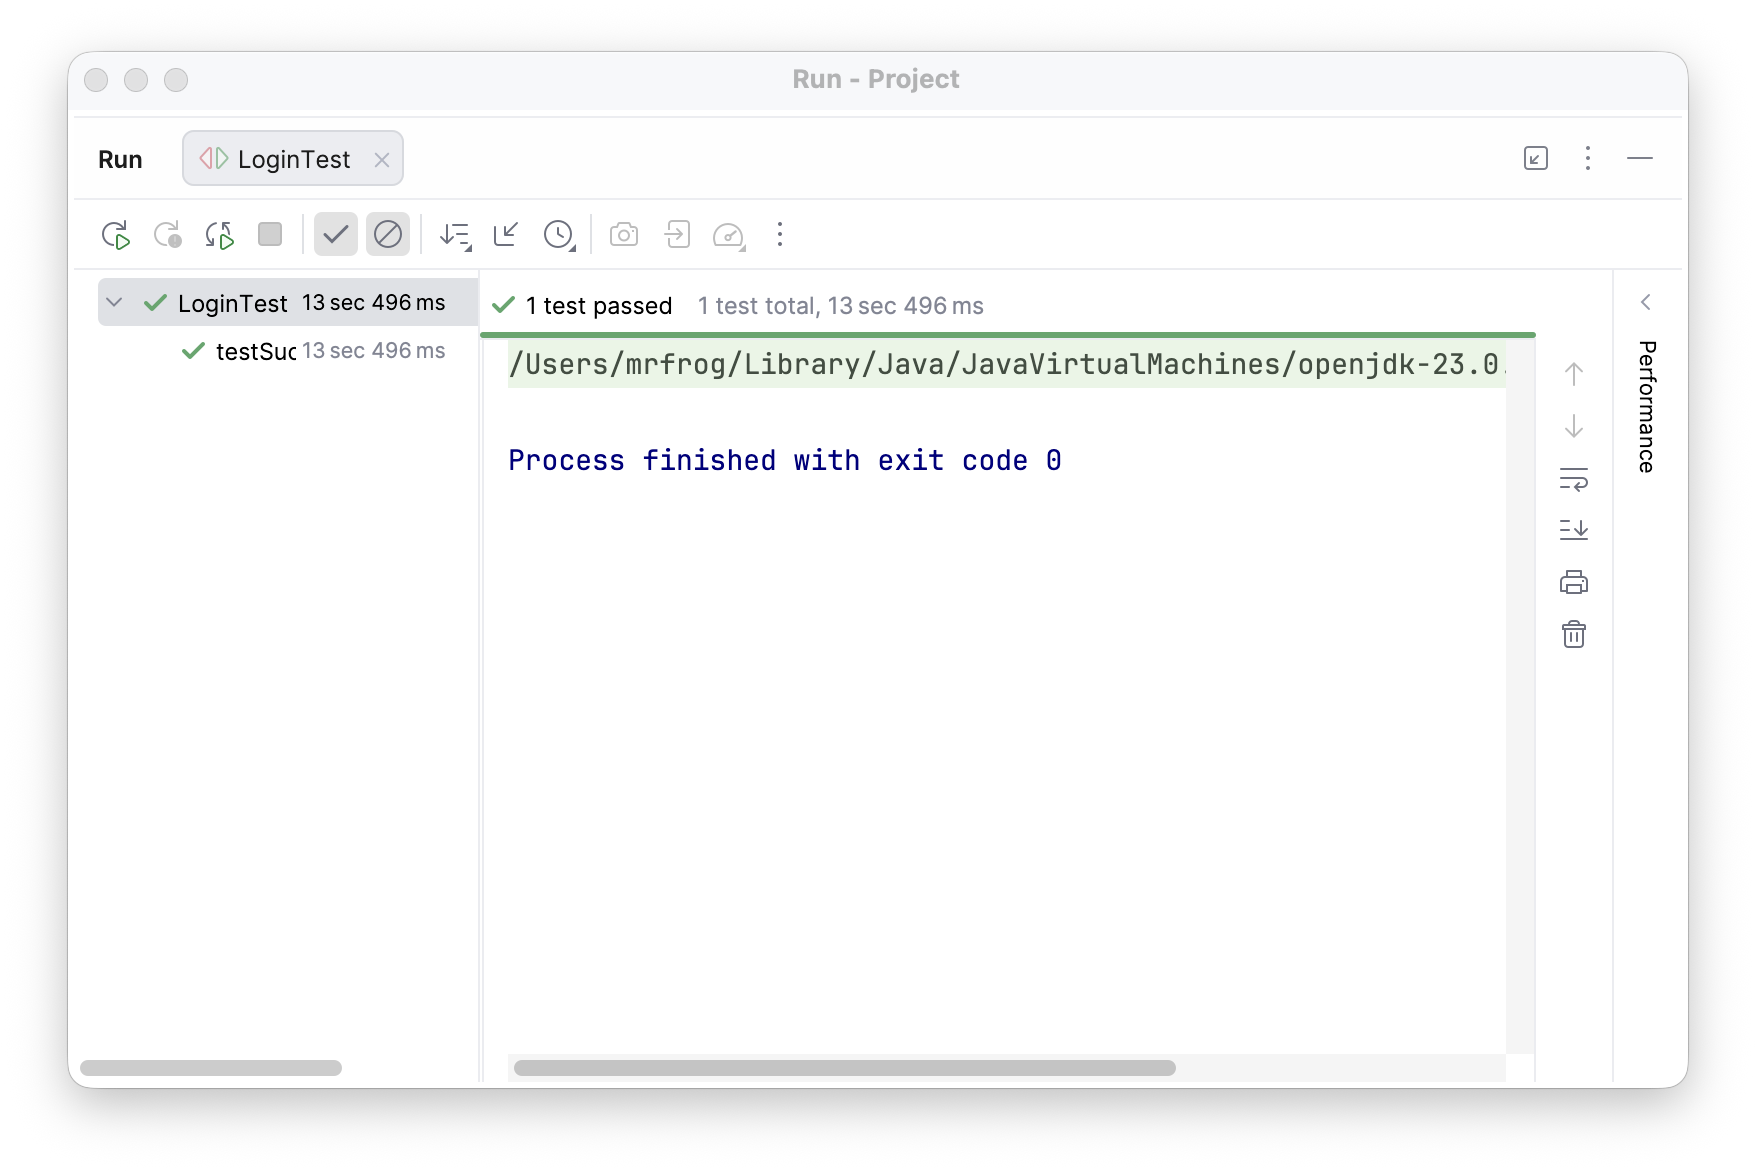
\includegraphics[width=0.9\textwidth]{screenshot step/Tugas_test_result.png}
    \caption{Bukti Hasil Eksekusi Selenium Tugas POM Berkelanjutan}
\end{figure}

\section*{Repository}
Akses kode lengkap untuk praktikum Pertemuan 10 ini dapat ditinjau dan ditarik versinya melalui GitHub Repository terkait yang berisikan struktur modular sistem.
\begin{center}
    \href{https://github.com/januarsyah901/PPPL}{GitHub Repository Base}
\end{center}

\clearpage

%======================================================================
\chapter{Kesimpulan}
%======================================================================

Berdasarkan praktikum yang telah diinisiasi pada Pertemuan 10, adopsi dari pola arsitektur \textit{Page Object Model} (POM) secara masif mentransformasi tatanan pengkodean \textit{Quality Assurance} menjadi rapi, kohesif, dan skalabel. Modifikasi skrip pengujian memisahkan elemen manipulatif \textit{web browser} ke dalam domain \textit{Page Object} tunggal, meminimalisir secara drastis redundansi tumpukan pendefinisian \texttt{WebElement} berulang. 

Dalam skala proyek yang meluas, utilisasi skema \textit{Centralized Locators} berdampingan erat dengan generalitas interaksi pada \texttt{BasePage}. Struktur penyelesaian ini memastikan apabila antarmuka visual sebuah aplikasi mengalami restrukturisasi format di level rekayasa front-end, perawatan (\textit{maintenance code}) Selenium cukup terpusat pada satu lokasi deklarasi \texttt{By selector}-nya semata tanpa mencemari stabilitas rentetan instansiasi test spesifik lainnya.

\end{document}
